\documentclass{beamer}
\usetheme{Madrid}
\usecolortheme{whale}

\usepackage{amsmath,amssymb,amsfonts}
\usepackage{graphicx}

\title[75MW Solar Plant Integration]{Integration of 75MW Solar PV Plant:\\Transmission System Design Analysis}
\author{Brent Dickinson \and Tianci Xie}
\date{December 10, 2024}

\begin{document}
	
	\begin{frame}
		\titlepage
	\end{frame}
	
	\begin{frame}{Project Objectives}
		Design transmission system modifications to:
		\begin{itemize}
			\item Integrate 75 MW solar PV at NEWSOLAR substation
			\item Provide redundant transmission paths
			\item Resolve existing system violations
			\item Maintain stability under N-1 contingency
			\item Minimize total cost including 5-year loss reduction
		\end{itemize}
	\end{frame}
	
	\begin{frame}{Initial System Analysis}
		\begin{columns}[T]
			\begin{column}{0.4\textwidth}
				Base System Characteristics:
				\begin{itemize}
					\item Total load: 826.3 MW, 275.5 Mvar
					\item Generation: 837.7 MW from 10 generators
					\item System losses: 10.7 MW (1.3\%)
					\item Reactive support: -122.5 Mvar from 9 switched shunts
				\end{itemize}
			\end{column}
			\begin{column}{0.6\textwidth}
				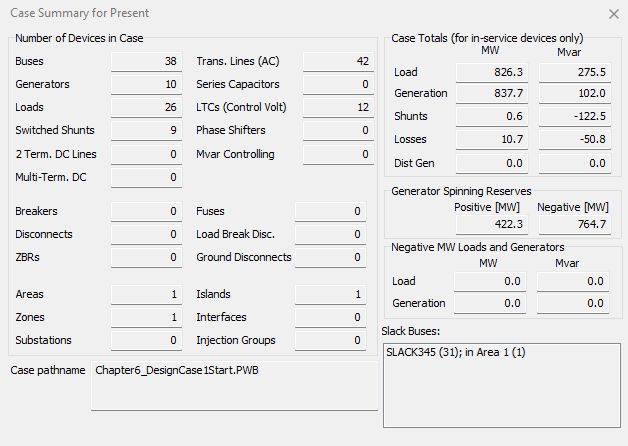
\includegraphics[width=1\linewidth]{figures/case_summary_existing}
			\end{column}
		\end{columns}
	\end{frame}
	
	\begin{frame}{Existing System Violations}
		\begin{table}
			\centering
			\begin{tabular}{|l|c|c|c|}
				\hline
				\textbf{Contingency} & \textbf{Flow} & \textbf{Limit} & \textbf{\%} \\
				\hline
				\textit{PINE138-PINE69 Xfmr:} & & & \\
				OAK69-BUCKEYE69 & 760.3 & 686.1 & 110.8 \\
				BUCKEYE69-APPLE69 & 454.2 & 418.4 & 108.6 \\
				\hline
			\end{tabular}
		\end{table}
		\centering
		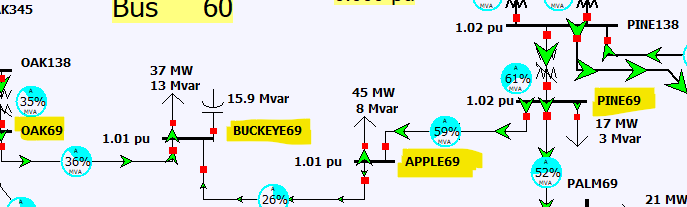
\includegraphics[width=0.7\linewidth]{figures/base_violations}
	\end{frame}
	
	\begin{frame}{Design Approach}
		\begin{itemize}
			\item Evaluate all possible connection configurations
			\item Compare 69 kV vs 138 kV options
			\item Start with shortest distance solution
			\item Use least expensive conductors initially
			\item Upgrade components only as needed
			\item Consider loss reduction benefits
		\end{itemize}
	\end{frame}
	
	\begin{frame}{Candidate Solutions}
		\begin{columns}[T]
			\begin{column}{0.4\textwidth}
				19 possible configurations evaluated:
				\begin{itemize}
					\item 69 kV options: \$5.94M - \$12.23M
					\item 138 kV options: \$14.37M - \$19.42M
					\item Shortest path: NEWSOLAR to BUCKEYE69 \& APPLE69 (12 km)
					\item Required upgrade - contingency violations
				\end{itemize}
			\end{column}
			\begin{column}{0.6\textwidth}
				\resizebox{\columnwidth}{!}{
					\begin{tabular}{|c|l|c|r|}
						\hline
						\textbf{Case} & \textbf{Destination} & \textbf{Total} & \textbf{Total Cost} \\
						\textbf{number} & \textbf{buses} & \textbf{distance (km)} & \textbf{(M\$)} \\
						\hline
						1 & BK69, AP69 & 12 & 5.94 \\
						2 & BK69, OAK69 & 19 & 8.53 \\
						3 & BK69, OAK138 & 19 & 14.37 \\
						4 & AP69, OAK69 & 19 & 8.53 \\
						5 & AP69, OAK138 & 19 & 14.37 \\
						6 & BK69, PIINE69 & 20 & 8.90 \\
						7 & BK69, PINE138 & 20 & 14.90 \\
						8 & AP69, PINE69 & 20 & 8.90 \\
						9 & AP69, PINE138 & 20 & 14.90 \\
						10 & BK69, MP69 & 21 & 9.27 \\
						11 & AP69, MP69 & 21 & 9.27 \\
						12 & OAK69, PINE69 & 27 & 11.49 \\
						13 & OAK69, PINE138 & 27 & 18.36 \\
						14 & OAK138, PINE69 & 27 & 18.36 \\
						15 & OAK138, PINE138 & 27 & 18.36 \\
						16 & OAK69, MP69 & 28 & 11.86 \\
						17 & OAK138, MP69 & 28 & 18.89 \\
						18 & PINE69, MP69 & 29 & 12.23 \\
						19 & PINE138, MP69 & 29 & 19.42 \\
						\hline
					\end{tabular}
				}
			\end{column}
		\end{columns}
	\end{frame}
	
\begin{frame}{Final Solution Design}
	\begin{columns}[T]
		\begin{column}{0.5\textwidth}
			\begin{minipage}{\columnwidth}
				\resizebox{\columnwidth}{!}{
					\begin{tabular}{|l|r|}
						\hline
						\textbf{Component} & \textbf{Cost (M\$)} \\
						\hline
						NEWSOLAR-BUCKEYE Line & 2.97 \\
						NEWSOLAR-APPLE Line & 2.97 \\
						BUCKEYE-ORANGE Line & 3.71 \\
						Loss Savings (1.2 MW) & -3.15 \\
						\hline
						\textbf{Total} & \textbf{6.50} \\
						\hline
					\end{tabular}
				}
			\end{minipage}
			
			\vspace{1em}
			\begin{minipage}{\columnwidth}
				Key Features:
				\begin{itemize}
					\item All new lines use Rook conductor
					\item Redundant paths to NEWSOLAR
					\item No existing line upgrades needed
				\end{itemize}
			\end{minipage}
		\end{column}
		\begin{column}{0.5\textwidth}
			\includegraphics[width=\linewidth]{figures/finalschematic}
		\end{column}
	\end{columns}
\end{frame}

\begin{frame}{Loss Reduction Analysis}
	\begin{columns}[T]
		\begin{column}{0.4\textwidth}
			\begin{itemize}
				\item Base case losses: 10.7 MW
				\item Final configuration: 9.5 MW
				\item Savings: 1.2 MW
				\item 5-year energy savings: 52,560 MWh
				\item Economic value: \$3.15M at \$60/MWh
			\end{itemize}
		\end{column}
		\begin{column}{0.6\textwidth}
			\includegraphics[width=1\linewidth]{figures/finallosses}
		\end{column}
	\end{columns}
\end{frame}

\begin{frame}{Conclusions}
	\begin{itemize}
		\item Optimal solution: 69 kV connections to BUCKEYE \& APPLE, plus new BUCKEYE-ORANGE line
		\item Strategic BUCKEYE-ORANGE connection eliminates need for OAK-BUCKEYE upgrade
		\item Substantial loss reduction: 1.2 MW
		\item Total cost \$6.50M including loss savings
		\item Meets all reliability and redundancy requirements with simpler implementation
	\end{itemize}
\end{frame}
	
	\begin{frame}{Live Demo - Tianci}
		\centering
		\Large{Thank you}
	\end{frame}
	
\end{document}